\section{Результаты измерений}
Без приложения внешней силы широскоп покоится, т.к. все внешние силы и их моменты
скомпенсированы. При нажатии на рычаг гироскоп поворачивается в плоскости, перпендикулярной
направлению приложенной силы.

Измерим время и угол, на который повернётся ось гироскопа вокруг верикальной оси, опустившись
при этом на 10 градусов. $l=121\,\text{мм}$

\begin{table}[!ht]
    \centering
    \begin{tabular}{|l|l|l|}
    \hline
        $m,\;\pm 0{,}1\;\text{г}$ & $t,\text{с}$ & $\varphi,\;\pm 2^{\circ}$ \\ \hline
        341.7 & 274.85 & 3270 \\ \hline
        271.9 & 343.38 & 3240 \\ \hline
        219.5 & 378.22 & 2880 \\ \hline
        175.6 & 414.5 & 2520 \\ \hline
        141.7 & 440.16 & 2160 \\ \hline
        115.8 & 465 & 1860 \\ \hline
        92.6 & 448.31 & 1440 \\ \hline
        76.1 & 577.18 & 1530 \\ \hline
        56.7 & 576.59 & 1140 \\ \hline
    \end{tabular}
\end{table}

Параметры цилиндра: $m=1616{,}7\,\text{г}$, $d=78{,}3\,\text{мм}$.
Период колебаний цилиндра $T_1=4{,}04\pm 0{,}05\,\text{с}$.
Период колебаний ротора $T_1=3{,}21\pm 0{,}05\,\text{с}$.
Момент иннерции цилиндра $I_0=\frac{md^2}{8}$.
Момент иннерции цилиндра $I=I_0\frac{T_2^2}{T_1^2}=\left(78\pm 4\right)\cdot 10^{-5}\,\text{кг}\cdot\text{м}^2$.

\begin{figure}[ht!]
    \centering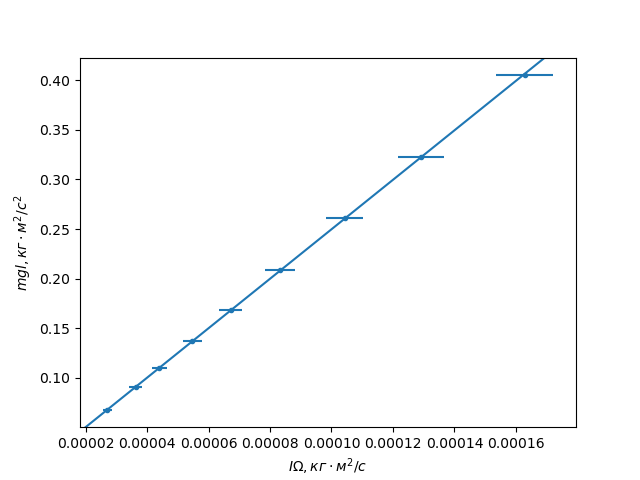
\includegraphics[width=0.8\linewidth]{img/plotk.png}
\end{figure}

$\omega_0=\frac{k}{2\pi}=400\pm20\,\text{Гц}$.

Измерения осциллографом дают $\omega_0\approx 390\,\text{Гц}$

Трение в вертикальной оси можно оценить из времени опусания оси рычага:
\[M=\frac{\varphi_0}{2\pi t}I\omega_0\]
$\varphi_0=10^\circ$

\begin{table}[!ht]
    \centering
    \begin{tabular}{|l|l|}
    \hline
        $m,\;\pm 0{,}1\;\text{г}$ & $M,\text{кг}\cdot\text{м}^2/\text{с}^2$\\ \hline
        341.7 & $1.8\pm 0.1$ \\ \hline
        271.9 & $1.5\pm 0.1$ \\ \hline
        219.5 & $1.4\pm 0.1$ \\ \hline
        175.6 & $1.3\pm 0.1$ \\ \hline
        141.7 & $1.16\pm 0.09$\\ \hline
        115.8 & $1.1\pm 0.09$ \\ \hline
        92.6 & $1.14\pm 0.09$ \\ \hline
        76.1 & $0.89\pm 0.07$ \\ \hline
        56.7 & $0.89\pm 0.07$ \\ \hline
    \end{tabular}
\end{table}

Момент сил трения в оси ротора пропорционален угловой скорости, т.к. в смазке
возникает вязкое трение.
\[M=k\omega\]

Измерим зависимость частоты вращения от времени после выключения тока.
\begin{table}[!ht]
    \centering
    \begin{tabular}{|l|l|}
    \hline
        $\nu,\text{Гц}$ & $t,\text{с}$ \\ \hline
        390.4 & 0 \\ \hline
        381.2 & 30 \\ \hline
        373.3 & 60 \\ \hline
        364 & 90 \\ \hline
        354.9 & 120 \\ \hline
        345.7 & 150 \\ \hline
        336.8 & 180 \\ \hline
        328.1 & 210 \\ \hline
        319.7 & 240 \\ \hline
        311 & 270 \\ \hline
        302.7 & 300 \\ \hline
        294.7 & 330 \\ \hline
        286.8 & 360 \\ \hline
        279.2 & 390 \\ \hline
        271.5 & 420 \\ \hline
        264.1 & 450 \\ \hline
        256.7 & 480 \\ \hline
        249.4 & 510 \\ \hline
        242.4 & 540 \\ \hline
        235.3 & 570 \\ \hline
        228.5 & 600 \\ \hline
    \end{tabular}
\end{table}

\[k=\frac{I\ln\frac{\nu_0}{\nu}}{t}\]

\begin{figure}[ht!]
    \centering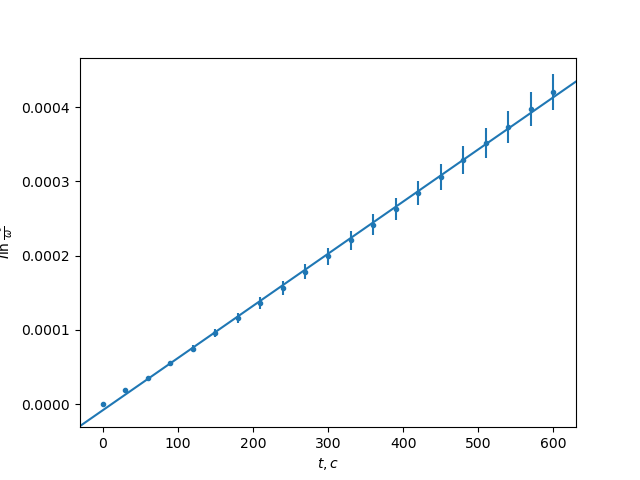
\includegraphics[width=0.8\linewidth]{img/pltm.png}
\end{figure}

$k=\left(703\pm 4\right)\cdot 10^{-9}\,\text{кг}\cdot\text{м}^2/\text{с}$

$M=k\omega_0=\left(1725\pm 99\right)\cdot 10^{-6}\,\text{кг}\cdot\text{м}^2/\text{с}^2$
